The submitted code is split into two libraries, each kept in a separate repository.
The first library, called \texttt{PerpleX-cpp}, contains the C++ wrapper code for Perple\_X and consists of both Fortran and C++ code.
The second, called \texttt{PerpleX-ASPECT}, predictably contains the plugin code that implements the wrapper inside of ASPECT and is written entirely in C++.
A diagram displaying the relations between the repositories as well as Perple\_X and ASPECT are shown in Figure~\ref{fig:dataflow}.
Alongside the source code, a wiki is provided giving useful information about things such as setting up a development environment on the Hamilton supercomputer, viewing the results in Paraview, and using Docker.

The justification for splitting the code into two repositories is twofold.
Firstly it ensures that the Perple\_X wrapper code is entirely general and the library can be used outside of ASPECT.
Secondly, it enforces a separation between the ASPECT code and the wrapper.
This is potentially valuable were the plugin code to be integrated upstream into the main ASPECT repository.

The code for both libraries is compiled using CMake.
CMake is a cross-platform build tool that can generate native makefiles and handle testing through CTest.
It was a requirement for the ASPECT plugin code as the ASPECT developers provide a CMake script that links the code to ASPECT and the underlying deal.II library.
However, it was very helpful to also compile the plugin code using CMake because integrating libraries is straightforward.

Regarding the code licensing, both Perple\_X and ASPECT are licensed under the GNU Public License (GPL) version 2.
In order for the submitted code to be compliant with these licences it has been licenced using the more modern GPL version 3.

\begin{figure}[ht]
    \centering
    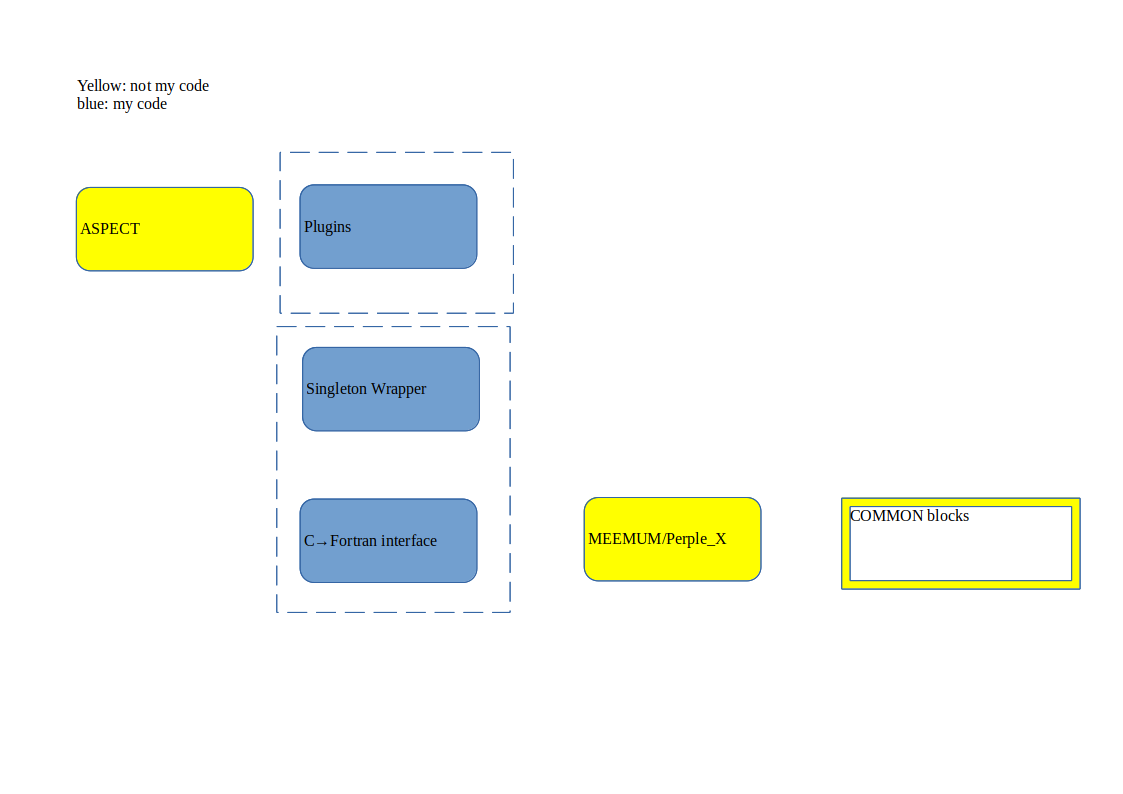
\includegraphics[width=\textwidth]{figures/dataflow.png}
    \caption{Diagram displaying the flow of data through the program. The blue blocks represent the new code and the yellow blocks represent the reused code.}
    \label{fig:dataflow}
\end{figure}

\subsection{Perple\_X C++ wrapper code}

The Perple\_X wrapper library presents two main functions to the user: one to initialise Perple\_X and the other to perform the MEEMUM computation and return the result.
It aims to abstract away to the greatest extent possible the complexities of dealing with the Perple\_X codebase.
For example, the only argument necessary to initialise the wrapper code is the path to the Perple\_X problem file and the only arguments needed to perform a subsequent calculation are the pressure, temperature and composition (which is just an array).

\subsubsection{Original Perple\_X source code}

Starting from the Perple\_X code and working up to the wrapper (see Figure~\ref{fig:dataflow}), the first component of the library is the Perple\_X source itself.
The decision was made to directly include the source code inside the repository rather than either encouraging the user to install Perple\_X themselves or retrieving via a URL.
The principle reason for this is reliability, Perple\_X receives frequent breaking updates and there is no easy way to access old versions so in order to ensure that the code remains in a usable state the source code is stored inside the repository.
The version used in the repository at the time of writing is 6.9.0.
Despite adding the code to the repository and tracking changes, the code has not been changed from the original Perple\_X code at all.
This is to try and minimise the amount of issues that will occur if at any point the Perple\_X version is ever upgraded.
Additionally the codebase is actually relatively small so inclusion does not create any significant overhead.
MEEMUM only depends on 8 (at the time of writing) source files and compilation occurs in well under a minute.

When Perple\_X is downloaded it comes with many files that compile to different executables other than MEEMUM as well as lots of thermodynamic database files and various README's.
To avoid confusion, only the necessary source files are included inside the repository.

\subsubsection{Fortran-to-C++ interface}

The basic concept of integrating Fortran code into C++ is very simple, all that is required is a C++ header file declaring the needed Fortran functions and variables using the correct symbols (e.g. the function \texttt{foo()} is normally represented with the symbol \texttt{foo\_} by the linker) and then the codes can be linked during compilation.
However, actually implementing this is far from straightforward: many of the data types are incompatible, array indexing starts from zero (C++) or one (Fortran) and arrays themselves are alternately row-major order (C++) and column-major order (Fortran).

This problem is compounded in Perple\_X by the sheer number of global variables, both constant PARAMETER's and COMMON blocks that are used by the program.
The source code contains a 400 line file called \texttt{perplex\_parameters.h} that contains the program parameters as well as lots of frequently used COMMON blocks.
If one were to write a C++ wrapper then this file would need to be converted into a C++ header as well as any MEEMUM specific code.

This was the approach taken previously by ???. A Python script was written that `compiled' the Fortran parameter file into a C++ header permitting linking.

However, this approach has a number of serious drawbacks: (a) whenever Perple\_X is upgraded this script must be re-run (b) the process is complex and hard to debug in case errors occur (c) the resulting header file is hard to read.

To solve these issues, an additional Fortran file was included in the codebase to `sanitise' the interface.
It provides a small number of property getters and setters as well as a largely verbatim copy of the MEEMUM subroutine, only altered to eliminate any calls for user input and split into initialise (called once) and compute (called many times) sections.
Arguments are passed by value (C-like) and only single values are passed (excluding strings), avoiding any complexities involved with arrays.

An additional advantage of this approach is readability.
Being written in Fortran 77, Perple\_X has a 6 character limit on its variable names which can make it very hard to follow what the variables and functions do.
The new interface code was not so restricted allowing for much more verbose function names.

\subsubsection{Singleton wrapper}

Although the basic interface described above is a significant improvement on previous approaches, it is still fairly limited.
Only basic data types are accepted and its use requires interacting with global variables, something that is considered poor software development practice.

Our solution to both these problems is the creation of a \texttt{Wrapper} class.
The class presents initialise and compute methods to the user and hides the details of interfacing with the Fortran at all.
It additionally permits the use of more complex data types, such as \texttt{std::vector} and \texttt{std::string} that are in common use in ASPECT.
An object-oriented solution was chosen because Perple\_X consists of both functions and data, making it a good idea to group them together into a class.

The class also implements the \textit{singleton pattern}, that is, only a single instance of the class may ever exist at the same time.
This approach was taken in order to prevent concurrent accesses to the Perple\_X data structures that are global.

During the project, it was noticed that many computations were being done with either identical or almost identical inputs. 
It therefore made sense to store the most frequently used results and use them if the inputs are sufficiently similar.
A cache was implemented using a least recently used (LRU) eviction policy.
A flowchart detailing the decision process for a LRU cache is shown in Figure~\ref{fig:cache_flowchart}.

\begin{figure}[ht]
    \centering
    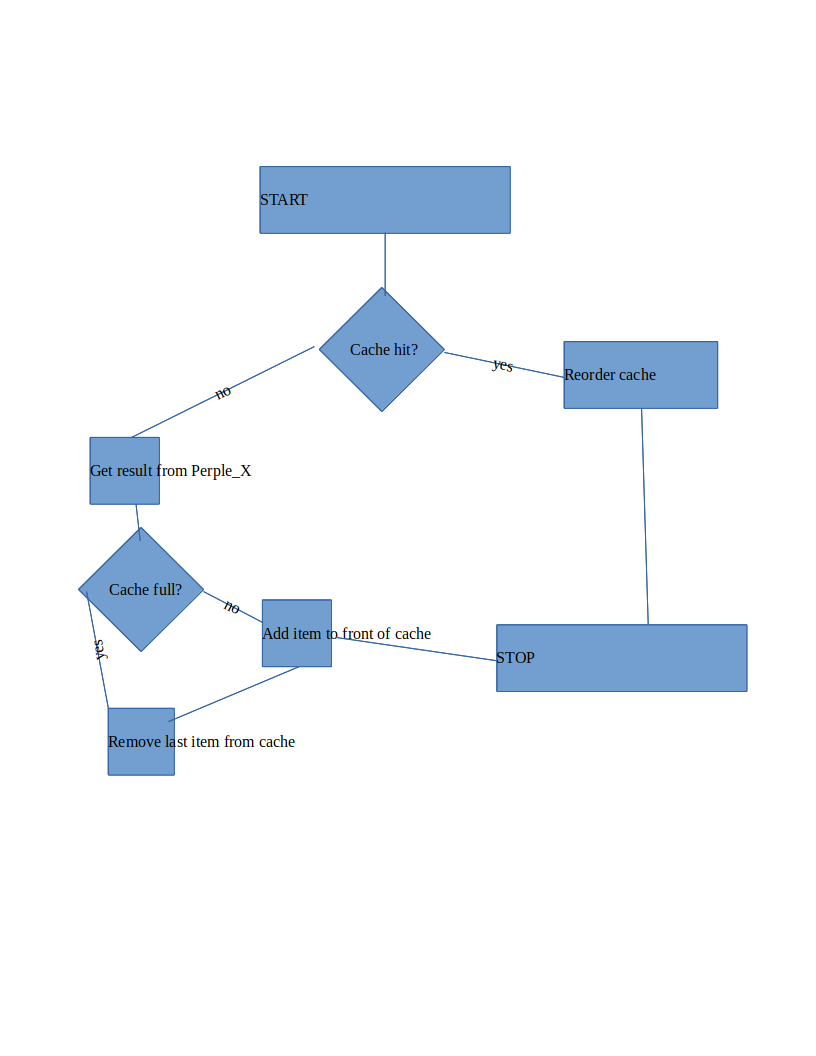
\includegraphics[width=\columnwidth]{./figures/cache_flowchart.png}
    \caption{Flowchart showing the decision process for the least recently used (LRU) cache used by the \texttt{Wrapper} class.}
    \label{fig:cache_flowchart}
\end{figure}

\subsubsection{Testing}

The library is tested using the Google C++ unit testing framework Google Test.
For the Fortran-to-C++ interface and singleton wrapper class, the tests consist largely of a direct comparison between the results of the function calls and previously collected MEEMUM output for a quick-to-run sample data set.

\subsubsection{Parallelism}

Perple\_X is not designed for parallel execution and as such the library is not thread-safe. 
However, there are only several methods that are exposed to the user so it would be straightforward to add locks to these methods making them thread-safe.
In contrast, the code is entirely suitable for parallel use in a distributed memory environment (i.e. MPI) because the global state is still local to each processor.
MPI is the primary parallelisation method used within ASPECT and so thread-safety was not considered a necessary feature of the library.

\subsection{ASPECT plugins}